\documentclass[a4paper]{book}
\usepackage[utf8]{inputenc}
\usepackage[margin=3cm]{geometry} % For smaller margins
\usepackage{appendix} % For appendix support
\usepackage{tikz, pgfplots} % For the skill outcome graph
    \pgfplotsset{width = \textwidth, compat = newest}
\usepackage{graphicx} % For advanced picture insertion
\usepackage{pdfpages} % For inserting PDFs
\usepackage{multicol} % For supporting multi-columnar tables
\usepackage{tcolorbox} % For coloured info boxes
    \tcbuselibrary{skins}
    \tcbset{colback=brown!10, fonttitle=\scshape}
\usepackage{textcomp} % For the interrobang
\usepackage[sc,sf,bf]{titlesec} % for custom titles
\usepackage{sectsty} % for section styles
\usepackage{fancyhdr} % for "fancy" headers
\usepackage[notmath]{sansmathfonts} % for a sans-serif small-caps font
 
%%%%%%%%%%%%%%%%%%%%%%%%%%%%%%%%%
%% CHAPTERS & SECTION HEADINGS %%
%%%%%%%%%%%%%%%%%%%%%%%%%%%%%%%%%


% Simplifies chapter titles
% No longer says
% Chapter 2
% Game Creation
% but instead simply
% 2 Game Creation
\titleformat{\chapter}[hang]
{\sffamily\bfseries\scshape\Huge}
{\thechapter\quad}{0pt}{}{}

% Removes unnecessarily large margin above chapter title
\titlespacing*{\chapter}{0pt}{-\topskip}{40pt}

% Set the remaining titles to be sans serif and small caps
\allsectionsfont{\sffamily\scshape}

%%%%%%%%%%%%%%%%%
%% THUMB INDEX %%
%%%%%%%%%%%%%%%%%

\renewcommand{\chaptermark}[1]{\markboth{\textsc{\thechapter\ #1}}{}}

%%%%%%%%%%%%%%%%%%%%%%%
%% CUSTOM TEXT BOXES %%
%%%%%%%%%%%%%%%%%%%%%%%
\newtcolorbox{note}{
    enhanced, % enable advanced settings
    left = 10mm, % pushes text away from the left edge by 10mm
    sharp corners, % disables rounded corners
    rounded corners = southeast, % "round" the bottom right corner
    arc is angular, % make the "round" corner an angle
    arc = 3mm, % controls corner cut
    boxrule=0.6pt, % sets box line thickness
    underlay={%
        \path[fill=tcbcolback!80!black] ([yshift=3mm]interior.south east)--++(-0.4,-0.1)--++(0.1,-0.2); % triangle
        \path[draw=tcbcolframe,shorten <=-0.05mm,shorten >=-0.05mm] ([yshift=3mm]interior.south east)--++(-0.4,-0.1)--++(0.1,-0.2); % triangle edge
        \path[fill=gray!50!black,draw=none] (interior.south west) rectangle node[brown!10]{\Huge\bfseries \textinterrobang} ([xshift=8mm]interior.north west);
    },
    drop fuzzy shadow % adds drop shadow
}

\newtcolorbox{example}{
    enhanced,
    title = Example,
    before upper={\parindent15pt\noindent} % add paragraph indentation
}

\title{Siren - Simple RPG Engine $\beta1.1.0$}
\author{By Niko Lepka}
\date{\today}

\begin{document}

\maketitle

\chapter*{Preface}
\section*{What is Siren?}
Siren, the \textbf{Si}mple \textbf{R}PG \textbf{En}gine, is a free and open source RPG system that aims at being simple and easy to learn without also compromising on the expressiveness of the system.

An RPG engine, much like a video game engine, is a framework on which you can build your own system. If any of the rules in this seem like they don't \textit{quite} fit what you need, you're free to change them for your campaign

\section*{What are RPGs?}
Role Playing Games, or RPGs for short, are games in which you take the role of some character and act in their stead.
You may know this from video games, where you play some adventurer in a medieval land full of magic and dragons; or where you play a person that's trying to survive in a nuclear wasteland, fighting mutants and warring factions.
But RPGs date back before that.

Traditional RPGs, also known as \textit{Tabletop RPGs} or \textit{Pen and Paper RPGs} date back to the early 1970s.
It's a social game played with a group of friends around a table, mutually telling a common story of great adventure, mysticism, space warfare or whatever they can come up with.

\section*{Who is this for?}
Some role-playing systems have hundreds of books and rules, so many so that it's hard to remember them all, and valuable playtime is spent looking up rules. 
While other systems have so few and vague, that a lot of playtime is spent arguing about which rules apply to a given situation.

Siren is made for those players who wish to have a small yet precise set of rules that can be used in every type of story, whether it's a grand space opera, or high fantasy, Siren's got you covered.

\section*{Where can I contribute?}
You can contrinute to Siren on https://github.com/ElectricCoffee/SirenRPG.
Guidelines for how to contribute are available on the page.

\section*{Conventions}
This book uses standard RPG dice notation, which looks like this: $AdX\pm L$, where $A$ is the number of dice, $X$ is the number of faces on the die, and $L$ is the value added or subtracted after the roll, so $3d6+8$ means roll three six-sided dice, and add 8 to the result.
\paragraph{Note} Notes are displayed like this, and often convey important information to the player or GM regarding a certain mechanic.
\paragraph{Example} Examples are displayed like this, and show a situation in which something is used.

\newpage
\section*{Special Thanks}
Special thanks to the lovely individuals who've helped out with the project:
\begin{center}
    \begin{tabular}{cccc}
        Aleksander Øglænd & Christian J. Martinsen & Marco L.L. Olsen & Morten M. Rasmussen \\
        Patrick A. & Thomas G. McCollin \\
    \end{tabular}
\end{center}

\section*{Licence}
This work is licensed under the Creative Commons Attribution-ShareAlike 4.0 International License.
To view a copy of this license, visit http://creativecommons.org/licenses/by-sa/4.0/ or send a letter to Creative Commons, PO Box 1866, Mountain View, CA 94042, USA.

\tableofcontents

\chapter{Getting Started}
\section{What You Need}
\begin{enumerate}
    \item \textbf{Three to six players.} One of which will have to be the Game Master (GM).
    \item \textbf{Character sheets.} One per player. Additional paper is encouraged, but not required.
    \item \textbf{GM sheet.} Special sheet for the Game Master.
    \item \textbf{Dice!} At least 3d6 per player, more is not necessarily required, but encouraged.
\end{enumerate}

\subsection{What's a Game Master?}
The Game Master is the special player in a game that directs the flow of the adventure.
The GM is responsible for narrating, setting up obstacles, and role-playing the Non-Player Characters (NPCs) that the players have to face throughout their adventures.

As a GM, the world is at your discretion. 
You roll the dice for everyone that isn't controlled by the players, you set the tone and mood of the environment, and you create the scenarios that will shape the decisions of the players.
You also get to set the difficulty of the obstacles at hand.

\subsection{The Role of the Player}
The player's role is to play their character, and face the trials imposed by the GM.
As a player, you control one of the protagonists in the story that the GM is telling, you make their choices and roll their dice to see how well they perform certain tasks.

\section{Performing Actions}
Actions are what usually drives the plot in an RPG, whether it's talking to an NPC or performing great heroic feats, it's all actions.

Some actions have a chance of failure, and thus require you to roll your dice (typically 3d6) to see if you succeed or not. 
These are performed as \textit{Skill Rolls} and are covered more in depth in chapter \ref{chap:skills}. 
The success or failure of this roll decides the fate of your character.

Other actions succeed automatically, and do not require a skill roll, unless there's a very good reason that there should be.
Imagine having to roll your dice every time you wanted to talk to an NPC or walk down the street. 
Unless your character has crippling social anxiety or completely lacks a balance, it's assumed that these sorts of things are automatically successful.

\chapter{Game Creation}
\section{Telling a Story Together}
First and foremost, the point of playing an RPG is telling a story together, how you manage to go about doing so is completely up to you.
Creating a good story for your players to interact with can be a bit difficult at times, but it is absolutely doable.
Let your imagination run wild and see what you can come up with!
Generally speaking you need a few things: A setting, a scale, a plot, and some NPCs.

\section{Setting}
The setting is one of the most important aspects of your game.
It determines everything from whether or not magic exists, to things like alien races, or level of technology.

Do you want to make 1940's style Noire story set in the distant future in a city that spans an entire planet? Go for it!
The most important thing, is that you---as the GM---can keep track of the setting, and keep it somewhat consistent.
Consistency is important so that things don't feel out of place. 
Don't be afraid to break consistency if you want to surprise or weird your players out.
It's your game world, make it however you want it.

\section{Scale}
When creating a game, it's also important to keep the scale of it all in mind.
Do you want a giant flourishing world filled to the brim with characters and opportunities on every corner? 
Or do you instead want something small and personal that can be wrapped up in a few sessions, but leaves a deep and profound impact on the players?
It's all up to you.
Just remember not to bite over more than you can chew, since bigger worlds tend to also require more work put into them.
It's easy to create this massive world and get lost in it.

\section{Plot}
What is a story without issues to resolve? Like any good movie or video-game, the story needs a plot-line.
Is a big evil corporation trying to take over the world?
Is a secret society conspiring against the general population?
Maybe a horde of dragons are stealing all the magic in the world for themselves in preparation for an upcoming war.

It's up to you, make it good.

\section{Non-Player Characters (NPCs)}
What is a world if there aren't anyone in it?
Just like the players need characters, so does the game world.
It's important to remember not only to make major plot-related NPCs, like a spy in the organisation you're trying to infiltrate, or the big bad guy that is foiling your plans at every step.
But minor NPCs like the slew of goons you want your players to fight, or that one one-off clerk at the shop that the players want to interact with.

NPCs generally come in those two flavours: Major and Minor.
Major NPCs are best created with a full character sheet, like the players, but minor NPCs can make by with just the most important stats written down.
\chapter{Character Creation}
Character creation is perhaps one of the most important aspects of an RPG.
How you design your character impacts how the game is going to be played.
This chapter is meant as a guide to help you through creating your character in Siren.

\section{Use Your Imagination}
Make your character yours.
Think of a back-story for them, give them a reason to exist in the world you're playing in.
If you are unsure about what works in the setting, ask your GM for help; after all, they're the one curating the game.
Work with the GM and the other players to create a character that best works for your game.

\paragraph{Note} The rest of the guide below is meant as a loose guide.
If the GM decides, any and all of the rules below can be changed to suit your particular game.

\section{The Character Sheet}
The character sheet comes in two pages.
Page 1 is the general stats page, which contains your traits, skills, and exploits.
Page 2 is the weapons and equipment page, which keeps track of your weapons, money, and loot.

\paragraph{Note} If you can't fit all your character's info, you can write them on the back of the character sheet!

\section{Building a Character}
\subsection{Experience Points}
To help you out, you'll get 100 XP to start out (The GM may decide to give more or less XP depending on setting).
These can be used to purchase skill bonuses and upgrade your traits if you so desire at the beginning of the game.
Check chapter~\ref{chap:char-prog} for more information about how XP works.

\subsection{Traits}
Each trait costs its own level in Experience Points, so bringing a trait up to level 3 requires paying 6 XP ($1 + 2 + 3$).
Note that you cannot exceed a trait level of 10.

The derived traits are calculated like this:

\begin{tabular} {r | l} 
\textbf{HP:} & $Con \times 2$ \\
\textbf{FP:} & $Con + Str$ \\
\textbf{MP:} & $Int \times Wis$ \\
\textbf{Def:} & Your character's Passive Defence score, see Chapter~\ref{chap:defence} for more info \\
\textbf{Parry:} & $Fighting / 2$, rounded down \\
\textbf{Speed:} & $Athletics / 2$, rounded down \\
\end{tabular}

\paragraph{Example} A character with the traits set up like this:

\begin{tabular}{r | l}
    \textbf{Agi} & 6\\
    \textbf{Cha} & 4\\
    \textbf{Con} & 5\\
    \textbf{Dex} & 6\\
    \textbf{Int} & 5\\
    \textbf{Str} & 4\\
    \textbf{Wis} & 3\\
\end{tabular}

Would cost 98 XP to build.
Note that a value of 5 is considered "average".

\paragraph{Note} Parry and Athletics are skills, covered in chapter~\ref{chap:skills}.
For Parry, the parrying ability depends on the fighting skill you're currently using.

\subsection{Skills}
Calculate your character's skills based on their traits as shown in the skill listing on your character sheet.
Think about what your character is particularly good at, these skills can be what your character specialises in.
These specialisations---or proficiencies---follow the \textit{Experience Points} section above.

\subsection{Exploits}
You may come up with up to one exploit during character creation (you have the option to add more as your character progresses).
Exploits are entirely player-defined, and are a way of personalising your character to fit your playstyle.
You can read more about exploits in chapter~\ref{chap:exploits}.

\subsection{Weapon Skills}
The weapon skills are separate from the general skills in that your character can specialise in any weapon under the sun if they so desire.
For this reason, you need to fill out the weapon stats for the given weapon yourself.
To help you out, we've included a weapon list in appendix~\ref{sec:weapons}, which provides a list of weapons and their relative stats.

\paragraph{Note} You cannot use a weapon skill unless you're also carrying a weapon.

\subsection{Magic Skills}
Like weapon skills, magic skills are separated for the same reason.
Check chapter~\ref{chap:magic} for more information about magic in general.

\subsection{Equipment}
The equipment section lists all the stuff you're carrying.
This is everything from armour and clothes, to loot, to weapons.

\subsection{Money}
Each box in the money section is for the currency carrying, and the lines next to the boxes are meant for the amount of said currency.
So if you're playing an international spy, the boxes could hold \textit{USD}, \textit{GBP}, \textit{EUR}.
And if you're playing in a fantasy setting, they could hold \textit{Gold}, \textit{Silver}, \textit{Bronze}.

\chapter{Traits}
\section{Introduction}
Traits are the aspects that define your character. 
These are things like their brains, their brawn, their fitness, etc. 
There are two different types of Traits in the game: \textit{Core Traits}, and \textit{Derived Traits}, which are special Traits derived from the core ones.
\section{Core Traits}
There are 7 core traits, each with an associated three-letter abbreviation.
Traits have an associated score, the score determines how good or bad your character will be at certain tasks during the game. 
You can find the core traits in Figure~\ref{fig:core_traits}.

\begin{figure}[!h]
    \centering
    \begin{tabular}{r | l}
        \textbf{Trait}  & \textbf{Description} \\\hline
        Agility      ($Agi$) & Movement and reaction \\
        Charisma     ($Cha$) & Ability to affect people \\
        Constitution ($Con$) & Health, stamina, and mettle \\
        Dexterity    ($Dex$) & Use of your hands and fingers \\
        Intelligence ($Int$) & Mental capability \\
        Strength     ($Str$) & Raw strength and muscle power \\
        Wisdom       ($Wis$) & Situational assessment and intuition
    \end{tabular}
    \caption{Core Traits}
    \label{fig:core_traits}
\end{figure}

\subsection{Agility (Agi)}
Agility represents your character's swiftness, manoeuvrability, and general fitness.
An agile character naturally lends themselves to speed, be it in terms of running or reaction time.

Agility is a core component in most physical skills; so whether your character is a professional boxer, an athlete, a bouncer, or a courier; Agility is the trait for you.

\subsection{Charisma (Cha)}
Charisma is your \textit{people skill}.
It represents your character's general ability to interact with, affect, and manipulate people.
A highly charismatic character can talk their way into or out of almost any situation, and as such Charisma is a core component in most of the social skills.

Whether your character is a sleazy con-artist, a performer, or a suave secret agent, Charisma is likely an important trait for you to consider.

\subsection{Constitution (Con)}
Constitution determines your character's health, their stamina, and their willpower, in other words: your character's general stubbornness.
Constitution is the core trait in everything to do with physical and mental health, and has a key role in a number of skills related to yours and other people's survival.

If your character is a medic, a ranger, or needs to tank a lot of hits, then Constitution is a good priority choice.

\subsection{Dexterity (Dex)}
Dexterity---or more accurately: \textit{manual} dexterity---governs your character's fine motor skills and ability to skilfully use their hands and fingers.
Intricate jobs like lock-picking, surgery, and watch-making all lend themselves nicely to a dexterous character, but coarser jobs that also require the use of your hands, like marksmanship and sailing also fall in this category.


\subsection{Intelligence (Int)}
Intelligence represents mental capacity, logical reasoning, and general academic prowess.
A highly intelligent character will have no trouble navigating academic resources and doing research; for this reason, most mental skills rely on Intelligence to some degree.

Good for characters who want to think their way out of and around problems.
Scholars, mages, and tacticians all benefit from a high Intelligence.

\subsection{Strength (Str)}
Strength represents the raw physical strength of your character.
Bulky and buff characters will naturally be strong, and are good for hitting hard and pulling the weight; this trait is key in some physical skills.

Bouncers, brutes, weight lifters, naturally benefit from a high Strength.

\subsection{Wisdom (Wis)}
Wisdom is your character's situational awareness, intuition, and general gut-feel.
For this reason, Wisdom applies to a wide variety of situations, as situational awareness and a good intuition will often be enough to get you through a lot of situations.

\section{Derived Traits}
The derived traits are all based on the core traits, and therefore cannot be chosen. 
You can find the derived traits on Figure~\ref{fig:derived_traits}.

\begin{figure}[!ht]
    \centering
\begin{tabular}{r | l}
    \textbf{Trait} & \textbf{Calculation} \\\hline
    Health  ($HP$) & $Con\times 2$ \\
    Fatigue ($FP$) & $Str + Con$ \\
    Mana    ($MP$) & $Int\times Wis$ \\
    Speed          & $Athletics / 2$\\
    Parry          & $Fighting/2 + \mathit{DfM}$\\
    Dodge          & $Speed + \mathit{DfM}$
\end{tabular}
    \caption{Derived Traits. (See Section~\ref{sec:defence} for $\mathit{DfM}$)}
    \label{fig:derived_traits}
\end{figure}

\subsection{Health (HP)}
Health represents a character's physical well-being.
If you have any past experience playing videogames or other RPGs, you know exactly what the purpose of Health is, but for those uninitiated, it is simply a measure of how close to dying your character is.
Worry not though, getting to zero HP does not instantly mean death!
More on that in Section~\ref{sec:health-points}.

\subsection{Fatigue (FP)}
Fatigue represents how hard your character can exert themselves.
Every point of fatigue has adverse effects on your character's ability to perform.
Get too fatigued, and your character faints from exhaustion.
You can read more about Fatigue as a mechanic in Section~\ref{sec:fatigue-points}.

\subsection{Mana (MP)}
Mana represents your character's magical potential and is used to cast spells (if the setting allows it).
Running out of mana runs the risk of exhausting your character, so use it effectively!
More about mana and how to use it in Section~\ref{sec:mana}.

\note If a certain setting calls for it, the MP can be used as ``Mental Points'' or ``Sanity Points'' instead of magical potential.
This is useful if you want to drain your players sanity over the course of campaigns that feature particularly horrifying things.
Though if you plan on using mana for that, consider calculating it as $Con \times Wis$ rather than $Int \times Wis$.

\subsection{Parry}
The Parry trait lets your character deflect an incoming attack using their fighting ability and/or a weapon.
This derived trait is a bit different from the others, in that it's based on two different skills \textit{Fighting (Light)} and \textit{Fighting (Heavy)}.
For this reason, the box on the character sheet is split in two.
More on parrying in Section~\ref{sec:defence}.

\note For all intens and purposes, parrying and blocking are treated interchangeably.

\subsection{Speed}
If playing with a battle-mat, the \textit{Speed} trait determines how many squares a character can move per turn.
More on that in Section~\ref{sec:movement}.

\subsection{Dodge}
The Dodge trait determines your character's ability to dodge out of the way of danger. 
By default it is equal to your character's Speed trait + the appropriate \textit{DfM}.
More about Dodge in Section~\ref{sec:defence}.

\section{Trait Saves}
Sometimes when a situation calls for it, you need to roll what's called a \textit{Trait Save}.
Trait saves are where you roll against your trait rather than your skill to affect the outcome of a certain situation.

A trait save is always $2 \times \mathit{affected\ trait}$, regardless of the trait.
Trait saves are different from \textit{Skill Rolls} (see Chapter~\ref{chap:skills}) in that they only make use of a single trait, and are not subject to modifiers.

\example Mark is on the brink of collapse.
He's lost a lot of blood in the battle against the mob boss.
His \textit{Constitution} is at 6, and needs to roll a \textit{Constitution Save} ($Con \times 2 = 12$) to not faint from blood loss.
He rolls a 2, a 6, and a 5, a total of 13. He collapses and faints.

\chapter{Skills} \label{chap:skills}
\section{Introduction}
Skills are the primary workhorse in the game. 
Whenever there's any situation that requires action, a player rolls against their skill plus/minus modifier. 
There are 19 different skills, as seen in figure \ref{fig:skills}. 
These skills reflect the different types of actions a player can perform during play.

\section{Skill Rolls}
The player rolls three six-sided dice (3d6) against their skill of choice, if the outcome is $\leq$ the skill level, it's a success, if not, it's a fail.
Rolling a 3, is an automatic success (regardless of level), and rolling an 18 is an automatic fail (also regardless of level).

\paragraph{Example} Say Alice wants to persuade a guard to do something stupid. Her \textit{Persuasion} skill is at 13. 
She rolls 3d6, and rolls a 1, a 5, and a 3, which is 9 in total. This means she successfully persuades the guard.

\begin{figure}
\centering
\begin{tabular}{r | c | c | l}
\textbf{Category} & \textbf{Skill}   & \textbf{Traits} & \textbf{Description} \\\hline
    Mental    & Academics        & $Int+Int$ & Use vast knowledge of a certain field.        \\
              & Investigation    & $Int+Wis$ & Searching for things and information.         \\
              & Magic            & $Int+Cha$ & Perform fantastical feats.                    \\
              & Perception       & $Int+Wis$ & The passive ability to spot things.           \\
              & Survival         & $Con+Int$ & Surviving in certain environments.            \\
              & Thievery         & $Dex+Int$ & Performing certain larcenous activities.      \\\hline
    Physical  & Athletics        & $Agi+Con$ & Perform a certain task that requires stamina. \\
              & Fighting (Heavy) & $Agi+Str$ & The ability to fight with heavy weapons.      \\
              & Fighting (Light) & $Agi+Dex$ & The ability to fight with light weapons.      \\
              & Physique         & $Con+Str$ & Any action that requires strength.            \\
              & Stealth          & $Agi+Wis$ & Sneaking around and acting unseen.            \\\hline
    Social    & Contacts         & $Cha+Int$ & Make and use connections with people.         \\
              & Insight          & $Cha+Wis$ & Sensing and social cues and motivation        \\
              & Nursing          & $Cha+Wis$ & Taking care of people                         \\
              & Persuasion       & $Cha+Wis$ & Manipulating people.                          \\\hline
    Technical & Crafting         & $Dex+Int$ & Making things with your hands.                \\
              & Shooting         & $Agi+Dex$ & Shooting or throwing objects.                 \\
              & Vehicle (Air)    & $Dex+Wis$ & Operating motorised air vehicles.             \\
              & Vehicle (Land)   & $Dex+Wis$ & Operating motorised land vehicles.            \\
              & Vehicle (Sea)    & $Dex+Wis$ & Operating motorised sea vehicles.             \\
\end{tabular}
\caption{Skill Listing}
\label{fig:skills}
\end{figure}
\newpage
\section{Proficiency Bonus \& Specialisation}
Your character can specialise in any number of different skills.
Specialising grants the skill a \textit{Proficiency Bonus} equal to the level of proficiency you have bought for that particular specialisation.
See chapter~\ref{chap:char-prog} for more info.

\paragraph{Note} Just because your character hasn't specialised in anything, does not mean they cannot perform it, it just means they don't get the proficiency bonus.

\paragraph{Example} Joyce is an Olympic runner, and has a \textit{Constitution} of 5, and an \textit{Agility} of 5; this gives her an \textit{Athletics} score of 10. 
As a runner, her specialisation in running grants her a $+2$ proficiency bonus to her \textit{Athletics} roll whenever she needs to perform a running task.
She rolls 11, but because her effective \textit{Athletics} score is 12 due to the bonus, she succeeds.

\newpage
\section{Skills in Depth}
\subsection{Mental Skills}
\subsubsection{Academics (Int + Int)}
The Academics skill, called \textit{Knowledge}, or \textit{Lore} in other games, is the skill of knowing things factually. 
This can be things your character has read, or something they've researched.
If your character needs to identify ancient writing, source herbs, design circuits, or have a meaningful discussion with an expert, this is the go-to skill.

\paragraph{Specialisations:}
\begin{center}
    \begin{tabular}{c|c|c|c}
        Maths & Physics & Chemistry & Theology \\
        Medicine & Literature & Linguistics & History \\
        Anthropology & Computer Science & Magic & Botany \\
        Geology & Astronomy & Quantum Physics & Computer Security \\
    \end{tabular}
\end{center}

\subsubsection{Investigation (Int + Wis)}
Investigation is the skill of actively searching for things and gathering information.
Whether your character is hunting for clues or digging through books, investigation is the skill to use.

\subsubsection{Magic (Int + Cha)}
Magic is the skill of performing fantastical things with power channeled through the body.
Whether it's chi energy, spiritual power, nanobots, genetic modification, or the essence of the universe that powers your abilities, it all falls under \textit{Magic}.

\paragraph{Specialisations:}
\begin{center}
  \begin{tabular}{c|c|c|c}
    Life  & Death & Construction & Destruction \\
    Earth & Water & Air & Fire \\
    Arcane & Black/Dark & White/Light & Temporal \\
    Divine & Diabolic   & Utility
  \end{tabular}
\end{center}
Magic is covered much more in depth in chapter \ref{chap:magic}.

\subsubsection{Perception (Int + Wis)}
Perception, called things like \textit{Notice} or \textit{Awareness} in other games, is the skill of using your senses to \textit{passively} notice what's going on around you.

\subsubsection{Survival (Con + Int)}
Survival is the skill of surviving; particularly in inhospitable environments.

\paragraph{Specialisations:}
\begin{center}
    \begin{tabular}{c|c|c|c}
        Desert & Tundra & Jungle & Island \\
        Prairie & Urban & Off-World & Space \\
        Under Water & Underground & Mountain & Arctic \\
    \end{tabular}
\end{center}

\subsubsection{Thievery (Dex + Int)}
Thievery is a catch-all term for general larcenous and/or criminal skills that (generally) involve thought and finesse.
These skills are regarded as such regardless of their actual use.

\paragraph{Specialisations:}
\begin{center}
    \begin{tabular}{c|c|c}
        Pick-Pocket & Lock-Pick & Sleight of Hand \\
        Alarm Deactivation & Hacking & Evidence Tampering \\
    \end{tabular}
\end{center}

\subsection{Physical Skills}
\subsubsection{Athletics (Agi + Con)}
Athletics, sometimes called \textit{Endurance} in other games, is a skill that has your character perform physically challenging things, often involving swiftness or stamina.
Tasks such as running, climbing, or swimming fall under here.

\paragraph{Specialisations:}
\begin{center}
    \begin{tabular}{c|c|c|c}
        Running & Climbing & Swimming & Jumping \\
        Acrobatics & Biking & Diving & Sailing \\
    \end{tabular}
\end{center}

\paragraph{Note} Sailing here refers to sailing a non-motorised sail or row boat. For motorised sailing, see the skill \textit{Driving}.

\subsubsection{Fighting (Heavy) (Agi + Str)}
This is the skill of melee fighting with heavy weaponry. Weapons such as clubs, mallets, war-hammers, axes, etc.\ fall under this skill.

\paragraph{Specialisations:}
\begin{center}
    \begin{tabular}{c|c|c|c}
        Mace & Club & Mallet & War Hammer \\
        Claymore & Baseball Bat & Pipe & Pipe Wrench \\
        Battle Axe & Two-by-Four & Odachi & Talwar \\
    \end{tabular}
\end{center}

\subsubsection{Fighting (Light) (Agi + Dex)}
This is the skill of melee fighting without weapons or with light weaponry. 
Weapons such as rapiers, short swords, lances, and knives fall under here.

\paragraph{Specialisations:}
\begin{center}
    \begin{tabular}{c|c|c|c}
        Rapier & Short Sword & Katana & Beam Sword \\
        Knife & Ice Pick & Baton & Brass Knuckles \\
        Fist (punching) & Foot (kicking) & Rolling Pin & Letter Opener \\
    \end{tabular}
\end{center}

\subsubsection{Physique (Con + Str)}
Physique, the raw strength counterpart to Athletics. 
This skill involves everything that requires strength.
Lifting, pulling, or pushing heavy objects are things that fall under here.

\subsubsection{Stealth (Agi + Wis)}
Stealth is the act of moving around unnoticed.
Tasks such as blending in, sneaking, and infiltrating all fall under here.

\subsection{Social Skills}
\subsubsection{Contacts (Cha + Int)}
Contacts is the skill of creating, maintaining, and making use of contacts.
So if your character needs to call a friend for help, or establishing a new connection with someone for use later, this is the skill for you.

\subsubsection{Insight (Cha + Wis)}
Insight, called \textit{Sense Motive} or \textit{Empathy} in other games, is the dual/opposite of \textit{Persuasion}. 
This skill is all about reading people and their intentions, and trying to figure out what they're up to.
So if you're suspecting a salesman is trying to scam you, or if you're trying to figure out if an unstable inmate is about to have a wild mood swing, this is the go-to skill.

\subsubsection{Nursing (Cha + Wis)}
The Nursing skill is all about taking care of animals and people and making them feel good.
A good nurse can have a positive effect on someone's mental and physical health, and in fact can help speed up their natural healing.
Essentially, one can think of nursing as non-magical healing.

\subsubsection{Persuasion (Cha + Wis)}
Persuasion is the skill for manipulating people for good or bad.
Whether you need to lure a guard away from his post, trick the evil sorcerer to reveal his secret plan, or strike a favourable deal with the mob boss, or maybe you just want to sit around in a pub cracking jokes, lightening the mood of the people around; this is the skill you want to use.

\paragraph{Specialisations:}
\begin{center}
    \begin{tabular}{c|c|c|c}
        Bargaining & Charming & Convincing & Inciting \\
        Seducing & Taunting & Provoking & Distracting \\
        Rapport & Deception & Bluffing & Intimidation
    \end{tabular}
\end{center}

\subsection{Technical Skills}
\subsubsection{Crafting (Dex + Int)}
The skill of making things, any hobby or task that involves producing something tangible with your hands belongs here.

\paragraph{Specialisations:}
\begin{center}
    \begin{tabular}{c|c|c|c}
        Paper Crafts & Origami & Carpentry & Woodworking \\
        Masonry & Smithing & Machining & Electronics \\
        Gadgeteering & Knitting & Casting & Sculpting \\
    \end{tabular}
\end{center}

\subsubsection{Shooting (Agi + Dex)}
Shooting is the skill of launching projectiles, whether it be by throwing, or launching them from a device.

\paragraph{Specialisations:}
\begin{center}
    \begin{tabular}{c|c|c|c}
        Throwing & Slingshot & Bow & Crossbow \\
        Pistol & Revolver & SMG & Rifle \\
        Assault Rifle & Cannon & Ballista & Trebuchet \\
        Mortar & Tank Turret & Helicopter Turret & Blowpipe
    \end{tabular}
\end{center}

\subsubsection{Vehicle, Air (Dex + Wis)}
The act of operating an airborne vehicle.

\paragraph{Specialisations:}
\begin{center}
    \begin{tabular}{c|c|c|c}
        Plane & Jet & Helicopter & Hot Air Balloon \\
        Commercial Liner & Zeppelin & Flying Car \\
    \end{tabular}
\end{center}

\subsubsection{Vehicle, Land (Dex + Wis)}
The act of operating land vehicles.

\paragraph{Specialisations:}
\begin{center}
    \begin{tabular}{c|c|c|c}
        Car & Truck & Tractor & Tank \\
        Train & Moped & Motorcycle & Hovercraft
    \end{tabular}
\end{center}

\subsubsection{Vehicle, Sea (Dex + Wis)}
The act of operating water based vehicles.
Note that sailing sail/row boats are Olympic disciplines, and thus fall under \textit{Athletics}.

\paragraph{Specialisations:}
\begin{center}
    \begin{tabular}{c|c|c|c}
        Jet-Ski & Motor Boat & Yacht & Cruise Liner \\
        Submarine & Hovercraft & 
    \end{tabular}
\end{center}

\newpage
\section{Contest of Skills}\label{sec:contest}
Situations arise, when your character needs to test their skills and prove their worth, this is done via a \textit{Contest of Skills}.
These contests come in three different variants: \textit{Passive}, \textit{Active}, and \textit{Tournament}.

\subsection{Passive Contest}
A passive contest arises when the character needs to overcome some passive obstacle. This could be things like walking a tightrope, picking a lock, leaping over a gap, etc.
The GM silently decides the level of difficulty by announcing a skill +/- a modifier that needs to be rolled.

\paragraph{Example} Astrid is running from her pursuers across the rooftops of ancient Rome, she needs to clear a particularly wide gap between the buildings. Astrid says \textit{``I'm jumping the gap''}, to which the GM replies \textit{``Roll Athletics -2''}. Astrid's Athletics skill is at 11, at -2, she must roll 9 or less to succeed. She rolls an 8 and gracefully leaps between the buildings.

\subsection{Active Contest}
An active contest is when the character is up against someone or something that actively works against them. Be it trying to pick-pocket a guard, an intense sword-fight, or playing chess against an opponent; all of this providing an \textit{active} resistance.

In an active contest, both parties roll against their most applicable skill, the outcome is judged as follows:

\begin{center}
    \begin{tabular}{c|c|c}
    \textbf{Character A} & \textbf{Character B} & \textbf{Winner}\\\hline
    Fail & Fail & The one failing by least \\
    Fail & Success & Character B \\
    Success & Fail & Character A \\
    Success & Success & The one succeeding by most
    \end{tabular}
\end{center}
If no one fails or succeeds more than the opponent, re-roll.

\paragraph{Example} Tom wants to sneak past a guard, Tom's \textit{Stealth} is at 9, he rolls 11, failing by 2 degrees. 
The guard's \textit{Perception} is at 10, but rolls 13, failing by 3 degrees. 
Tom failed less than the guard, thus successfully sneaking past them.

\subsection{Tournaments}
Tournaments are \textit{longer} contests of skills.
Tournaments are divided into rounds, whoever wins the most rounds wins the tournament.
Each individual round is a regular \textit{active contest}.

\chapter{Example Exploits}\label{app:exploits}
Trying to come up with new exploits in the heat of the moment can be hard.
This appendix exists to alleviate this pain and get the proverbial juices flowing!

Note that this by no means is an exhaustive list!
More can be added to fit the given campaign.
Also note that exploits should be limited somehow, so as to not be over-powered. What it means to be over-powered depends on context and setting. See Section~\ref{sec:exploit-balance} for exploit balancing.

\section{Tier One}

\subsection{Backstab (1 XP)}
\textit{You know the quickest way to a man's heart: through their back.}\\
You can attack with \textit{Stealth} instead of \textit{Fighting} provided your target isn't already aware of your presence.

\subsection{Bardic Charm (1 XP)}
\textit{You are an enchanting entertainer.}\\
When using the instrument of your choice, use $Int+Cha$ instead of $Int+Wis$ when casting spells.

\subsection{Desert Dweller (1 XP)}
\textit{You can instinctively search for food in a desert.}\\
You can use $Con + Wis$ instead of $Con + Int$ when looking for food with \textit{Desert Survival}.

\subsection{Intimidating Size (1 XP)}
\textit{You are big and burly, your size comes across as threatening.}\\
You can use $Cha + Str$ instead of $Cha + Wis$ to intimidate someone.

\subsection{Master Strategist (1 XP)}
\textit{Your training made you good at drawing plans.}\\
Get a $+2$ bonus on \textit{Academics} when drawing up a strategy.

\subsection{Red Tape Recorder (1 XP)}
\textit{You're fluent in government bureaucratic lingo.}\\ 
You can use $Int + Int$ instead of $Cha + Cha$ when trying to persuade government officials.

\subsection{Silver Tongue (1 XP)}
\textit{Your suave mannerisms have a way to woo even the most suspicious of people.}\\
You can use \textit{Persuasion} instead of \textit{Thievery} when trying to pick-pocket.

\section{Tier Two}

\subsection{Bloodlust (2 XP)}
\textit{``On a night of the hunt, it is no wonder that some resort to superstition.''}\\
When in melee combat, a roll of 4 or lower counts as an automatic success against non-human opponents.

\subsection{Body Builder (2 XP)}
\textit{No shoes, no shirt, you still get service.}\\
You can use \textit{Physique} instead of \textit{Persuasion} to distract people with your muscles.

\subsection{Computational Gunner (2 XP)}
\textit{You think before you shoot.}\\
You can use $Int+Wis$ instead of $Agi+Dex$ when you take time to aim a shot.

\subsection{De-Trapper (2 XP)}
\textit{They say no to trust a trapper with all their fingers, but they've never met you.}\\
Once per day, you may re-roll your least favourable die when disarming traps.

\subsection{Lucky Dodge (2 XP)}
\textit{Your dodging is phenomenal.}\\
Once per day, you may re-roll your least favourable die when trying to dodge.

\subsection{Now You See Me, Now You Don't (2 XP)}
\textit{An extensive background in Theatre, Espionage, or perhaps even pick-pocketing has gifted you with an nearly uncanny ability to assume another identity.}\\
While wearing a disguise, get a $+2$ bonus on \textit{Stealth} when trying to blend into a crowd.

\section{Tier Three}

\subsection{Blooddrunk (3 XP)}
\textit{``...Leave the hunting of hunters to me.''}\\
When in melee combat, a roll of 4 or lower counts as an automatic success.

\subsection{Machine Specialist (3 XP)}
\textit{If it has moving parts, you can figure it out.}\\
You can use \textit{Crafting} instead of \textit{Investigation} to deduce how any machine works regardless of prior familiarity.

\subsection{Mac's Back (3 XP)}
\textit{``The best way to beat a problem is to make it work for you.''}\\
\textbf{Requirements:} At least one \textit{Crafting} specialisation.

When deprived of the correct tools, materials, and/or workspace you are still able to make crafting checks so long as you are able to give an explanation to the GM of how your character did so.
Additionally, the maximum penalty on any \textit{Crafting} check is now $-2$.

\subsection{Right Behind You (3 XP)}
\textit{"And worst of all, he could be any one of us..."}\\
\textbf{Requirements:} \textit{Now you See Me, Now You Don't}.

Get a $+2$ bonus on \textit{Stealth} when trying to blend into a crowd.
If wearing a disguise, you instead get a $+4$ bonus.

\subsection{Red Tape Splicer (3 XP)}
\textit{You get up early, stay up late. You use a machete to cut through red tape.}\\
\textbf{Requirements:} \textit{Red Tape Recorder}.

Unconditional re-roll on \textit{Persuasion} against a government official.
Doing so damages your reputation with that agency.
(Removing this condition increases the cost to 4 XP.)

\subsection{Uncanny Dodge (3 XP)}
\textit{Your dodging is almost preternatural!}\\
\textbf{Requirements:} \textit{Lucky Dodge}.

Once per day, you may re-roll \textit{another} one of your unfavourable dice when trying to dodge.
You may either re-roll one die during two different encounters, or two dice during one encounter.

\section{Tier Four}

\subsection{The O'Neill Effect (4 XP)}
\textit{``How can you feel confined when you're in touch with the universe?''}\\
\textbf{Requirements:} \textit{Mac's Back}; military or paramilitary experience. 

You have a maximum penalty of $-3$ on crafting checks involving technology alien to you, and never suffers penalties when trying to disable such technology.
\chapter{Magic} \label{chap:magic}
\section{Introduction}
Some campaigns are set in a fantastical world, full of weirdness, improbable events, and of course: magic.
It is said that any technology that is sufficiently advanced, is completely indistinguishable from magic.
For this reason, we define the term \textit{Magic} to be a bit looser than traditionally.
So, whether we're talking beam sword wielding space wizards, battle mages, or even mutated people that gain power from sea slug juices;
if it seems to give super natural powers, it all just falls under this category.

\section{Basics}
The magic system consists of two things: spells and mana.
Spells are the things your magic abilities can do, and mana is the stuff that fuels the spells.
No mana, no spells.

\paragraph{Note} Spells are anything that is channeled through your body, regardless of how.
Whether the powers were given to you, or you were born with them, doesn't matter.

\section{Spells}
Spells come in many different forms: utility, healing, hurting, elemental, bionic etc.
Every spell has an associated mana cost, which consumes a bit of your total mana on each use (see Section~\ref{sec:mana}).

It's up to the players and the GM to decide the kinds of spells that exist within the game, and whether they're too game breaking or not.
Examples of spells include:
\begin{center}
  \begin{tabular}{c|c|c|c}
    Healing & Fireball & Lightning Strike & Mind Control \\
    Illusion & Freeze & Overload & Stop Time \\
    Push & Raise Dead & Create Golem & Shield
  \end{tabular}
\end{center}
Spells can be cast in three different ways:
\begin{enumerate}
\item On yourself.
\item Around you.
\item Away from you.
\end{enumerate}
Depending on the exact nature of that spell, these three casting methods can have vastly different effects.

\paragraph{Example} Casting a shield spell on yourself grants you protection.
Casting it around you creates a bubble around you that can shield yourself and your friends.
While casting it away from you can create a wall to shield something/someone further away.

\section{Mana}\label{sec:mana}
Every character has a mana pool $Int \times Wis$ in size, which represents the amount of magical potential your character can tap into without straining themselves.
In other words, if your character has 5 Int, and 6 Wis, they have 30 Mana Points (MP).
Every spell has an associated mana cost, and using it drains the mana pool accordingly.

\subsection{Running Out of Mana}
When you run out of mana, your can still cast spells!
However, instead of draining mana, your character will instead accumulate 2 Fatigue Points (FP) for every point of mana attempted to use.

\section{Casting a Spell}
Casting a spell requires two things: A skill roll, and enough mana.
Like all other skills, spells have four different outcomes, but being magic in nature, they act a bit differently from regular skills:
\begin{itemize}
\item \textbf{Critical Success.} The spell is performed at double strength, at no extra cost.
\item \textbf{Success.} The spell succeeds as intended.
\item \textbf{Fail.} The spell is not performed, but MP is still lost.
\item \textbf{Critical Fail.} The spell backfires at the GM's discression. All MP is lost.
\end{itemize}

\paragraph{Note} It's up to the GM or the setting to determine the difficulty of a spell.
The difficulty would be set as a $\pm$ skill modifier on the given spell.

\section{Charging a Spell}
A character can charge a spell if they wish to increase its power.
You can charge a spell by multiplying the amount of mana used the cast it;
this also multiplies its potency.
Every level of charging requires a new dice roll to maintain concentration, if any of them fail, the whole spell fails.

During combat, charging a spell takes multiple rounds.
If you want to cast a spell that is three times more powerful than normal, casting it takes 3 whole rounds of charging.
You lose any and all charge if you get distracted (damaged, tripping, etc.).

\paragraph{Example} Harold wants to burn a troll he and his party are fighting.
His fire spell consumes 5 MP, and decides to charge it for three turns.
At the beginning of his third turn, Harold unleashes an enormous cone of fire from the tip of his wand, consuming 15 MP in the process.

\section{Regaining Mana}
Mana is regained automatically over time.
About one point every 30 in-game minutes while not at rest,
a point every 10 minutes while relaxing,
and a full restoration after a good night's sleep.

If the setting allows it, mana potions can also help restore some of the spent mana.

\section{Acquiring New Spells}
You can cast any spell your character would logically be acquainted with within the boundries of the setting.
It is, however, up to the GM to decide the number of spells you are allowed to start out with.
Spell familiarity is determined through the skill proficiency system, see Chapter~\ref{chap:skills} for more info.

\paragraph{Note} Say your character finds a scroll with some mystical spell on it.
The scroll will give your character the knowledge of how to perform the spell, but they might still be unable to perform it well.
It will naturally take some time for your character to be familiar enough with the spell to perform it well.
Additionally, depending on the difficulty of the spell, it could be effectively uncastable at your character's skill level.

\chapter{Combat}
\section{Introduction to Combat}
Combat is a staple of most RPGs. 
It's intense, often exhilarating, and it gives the players a chance to strategise. Combat is essentially a series of \textit{Contests of Skill} (see section \ref{sec:contest}), but due to the nature of combat are naturally a bit more involved.
\subsection{Turns}
Combat is split into a number of turns, each turn represents about 6 seconds of in-game time, meaning 10 turns make up an in-game minute.

\paragraph{Note} One turn is the time it takes for every character to have had a go, not the time for each individual character.
\subsection{Turn Order}
To determine turn order, each player rolls $1d6+Athletics$. The turn-order is then ordered highest to lowest. Highest result goes first, lowest goes last. Any ties require a re-roll.

\paragraph{Example} Alice, Bob, and Clarice all roll for turn order. They have an athletics score of 9, 9, and 10 respectively. Alice rolls a 5, Bob rolls 3, and Clarice rolls a 6. Clarice goes first with 16, Alice is next with 14, and Bob is last with a score of 12.

\subsection{Simple Vs. Advanced Combat}
Siren supports two different styles of combat: \textit{simple}, and \textit{advanced}.

Simple combat is the most straightforward, and involves nothing more than your character sheets and your imagination. A drawn map to help visualise the space is nice, but not required.

Advanced combat, on the other hand, uses a battle mat divided into squares. This mat is used to communicate the exact position of characters and NPCs, and helps visualise movement and trajectories on the battlefield.

\newpage
\section{Simple Combat}

\subsection{Attack (Melee)}
\begin{enumerate}
    \item Roll against the appropriate weapon skill.
    \item If you succeed, the opponent gets to roll active defence (see chapter~\ref{chap:defence}).
    \item If the defence fails, or succeeds with less, roll for damage for the appropriate weapon.
\end{enumerate}

\subsection{Attack (Ranged)}
\begin{enumerate}
    \item Calculate effective skill level.
        \begin{enumerate}
            \item Target is \textbf{close}: Use base-skill.
            \item Target is at \textbf{medium} range: $Skill-3$.
            \item Target is \textbf{far}: $Skill-6$.
            \item Target is \textbf{very far}: $Skill-9$.
        \end{enumerate}
    \item Roll to attack, using the modified skill.
    \item If you succeed, target opponent may roll to dodge.
    \item If the dodge fails, roll for damage.
\end{enumerate}

\subsection{Defend}
Spend your turn doing nothing but defending. 
You get an additional $+2$ to your active defences (see chapter~\ref{chap:defence} for more). 
You may not attack during this turn.

\subsection{Long Action}
Any non-combat task that takes more than one turn is a \textit{long action}.
Examples of long actions could be picking a lock, untying someone, calling for backup, or applying bandages.

\subsection{Prepare Action}
Prepare an action to be triggered at a specific moment.
This can be waiting to hit someone until they're about to draw their sword, waiting for someone to turn around before hitting them in the head, or waiting for your opponent to reload their weapon before casting a spell.

\newpage
\section{Advanced Combat}
Advanced combat is much like simple combat, except it uses a battle mat. Because of this, the different possible actions in a turn are affected by this addition.

\subsection{Movement}
Particularly, the characters rely on their movement points to move about the battle mat.
Movement is 8-directional (see figure \ref{fig:directions}), and moving in any direction costs 1 movement point.

\begin{figure}
    \centering
    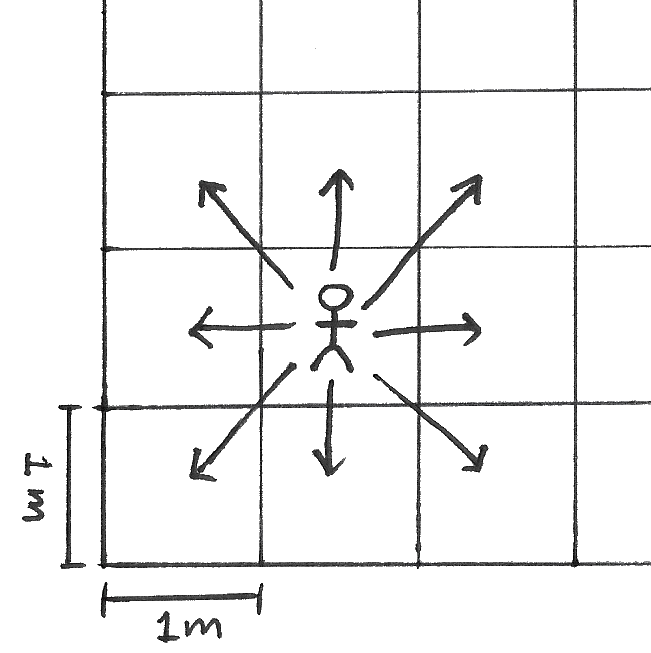
\includegraphics{graphics/directions-trans.png}
    \caption{The eight movement directions}
    \label{fig:directions}
\end{figure}

Your character can only move as far as their movement points allow, but you may choose to move a shorter distance if you so desire. Figure \ref{fig:movement} shows an example of a character moving 4 squares, which is worth 4 movement points.

\begin{figure}
    \centering
    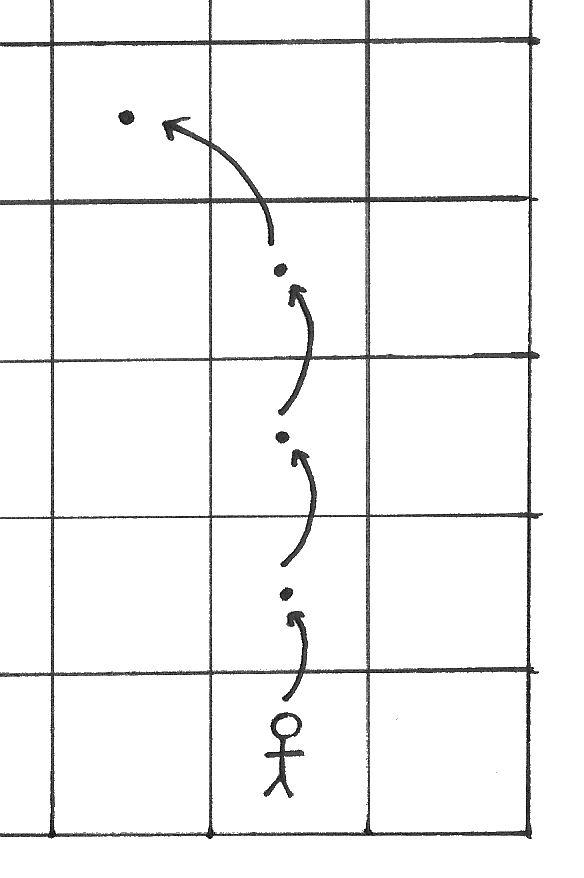
\includegraphics{graphics/movement-trans.png}
    \caption{Example of movement.}
    \label{fig:movement}
\end{figure}

\subsection{The Grid}
The battle mat is subdivided into a grid of squares. 
The in-game size of a square is $1m^2$, although the GM may scale it up or down as necessary.
The GM must alert the players of the scale if it differs from the standard $1m^2$.

\subsection{Actions}
\subsubsection{Long Action}

\subsubsection{Move \& Attack (Melee)}
\begin{enumerate}
    \item Move up to half your movement (rounded down) before or after attacking.
    \item Roll against the appropriate weapon skill.
    \item If you succeed, the opponent gets to roll active defence.
    \item If the defence fails, roll for damage for the appropriate weapon.
\end{enumerate}

\subsubsection{Move \& Attack (Ranged)}
\begin{enumerate}
    \item Move up to half your movement (rounded down) before or after attacking.
    \item Calculate effective skill level.
        \begin{enumerate}
            \item If target is within weapon's range, do nothing else.
            \item Subtract 3 points every time you exceed the range.
        \end{enumerate}
    \item Roll to attack, using the modified skill.
    \item If you succeed, the opponent may roll to dodge.
    \item If the dodge fails, roll for damage.
\end{enumerate}

\paragraph{Example} Will the Ranger is out hunting for his party. He spots a deer in the distance. His bow has a range of 100 metres, the deer is 300 metres away. This exceeds the bow's range twice ($2\times -3$ penalty). Will must roll $Longbow-6$ to succeed.

\subsubsection{Move \& Defend}
Move up to half your movement (rounded down) before defending. 
Spend the rest of your turn doing nothing else. 
You get an additional $+2$ to your active defences. 
You may not attack during this turn.

\subsubsection{Prepare Action}
Prepare an action to be triggered at a specific moment.
This can be waiting to hit someone until they step into the square in front of you, waiting for your opponent to reload their weapon before casting a spell, or waiting for a party member to stand in the square next to you before charging at the enemies.

\subsubsection{Relocate}
Move as far as your movement score allows and do nothing else.
Roll \textit{Athletics} to run, this doubles your range if you succeed.
If you fail you trip and fall prone.
If prone you may try to get up again on your next turn.

\section{Taking Damage}
It's not uncommon that you take damage during combat.
After all, having an angry wizard throw fireballs at you is going to hurt!
This section describes the ways in which damage is taken, and what the consequences are.
See chapter~\ref{chap:defence} for more info about damage resistance.

\subsection{Health Points}
Every character has a number of Health Points (HP).
The amount of HP a player has determines the player's level of consciousness:

\begin{center}
  \begin{tabular}{r | l}
    \textbf{HP Left} & \textbf{Effect} \\\hline
    $HP > 0$         & Alive and able to fight. \\
    $HP \leq 0$      & Roll against $2 \times Con$ to see if you faint. \\
    $HP \leq -HP$    & Roll against $2 \times Con$ to see if you die.
  \end{tabular}
\end{center}

\paragraph{Note} $-HP$ here refers to the negative of your max-HP.
In other words, if your character has 12 HP, $-HP = -12$
  
\subsection{Fatigue Points}
Fatigue is a different kind of damage.
One that affects you character more directly.
There are many different sources of fatigue: heat, starvation, dehydration, sleep deprivation, etc.

For every point of Fatigue Damage (FD) taken, your character suffers a $-1$ penalty on all skill rolls.

\begin{center}
  \begin{tabular}{r | l}
    \textbf{FD Taken} & \textbf{Effect} \\\hline
    $FD \geq FP/2$    & Roll against $FP - FD$ to see if you faint. \\
    $FD \geq FP$      & Immediately faint from exhaustion.
  \end{tabular}
\end{center}

\paragraph{Example} Charles has been walking the desert for the past five days.
The heat is getting to him, and he's taken 5 points of fatigue damage.
Charles has 10 FP, but due to the damage, he needs to roll 5 or less to not faint in the sand.
He rolls 9 and immediately collapses.

\section{Healing Damage}
Healing usually takes place \textit{outside} of combat, but can also be performed during combat as a \textit{Long Action}.
Healing takes time, and depending on the severity of the wound, the healing process takes a different amount of time.

The skill used for healing entirely depends on the task at hand.
Surgeries, anæsthetics, medicine, therapy, etc. all fall under the \textit{Academics} skill, while caretaking falls under \textit{Nursing}.
If however, it's automatic, then it depends on the effectiveness of that particular remedy.
That is, applying bandages or stitching a wound depends on the skill of the doer, while drinking a magic potion is dependent on the strength of the potion.

Healing comes in three different variants:

\begin{center}
  \begin{itemize}
  \item \textbf{Healing by mending.}
    This is the slowest form of healing, refers to any kind of healing performed via bandages, stitches, rest, or similar.\\
    Mending happens over the course of days or weeks.
  \item \textbf{Healing by potion.}
    The second-fastest form of healing, which refers to injecting or ingesting a substance that has regenerative properties. \\
    Potions heal over the course of minutes or hours.
  \item \textbf{Healing by magic.}
    The fastest form of healing, which refers to any procedure that facilitates instant healing, magic or otherwise.
  \end{itemize}
\end{center}

\paragraph{Note} Healing refers to both healing Health and Fatigue.
A cup of coffee, for example, is a fatigue-healing potion that takes about 30 in-game minutes to kick in.

\section{Defending \& Resisting Damage}\label{sec:defence}
Defending is performed by your character during the \textit{reactive phase} of combat.
This refers to actions like dodging, blocking, or parrying an attack.
Note that blocking and parrying are treated as the same type of action, since blocking with a sword and parrying with a shield mechanically act the same way.
More often than not, defensive actions have a lower chance of success, but also have a very high reward, as they make it possible to completely avoid all damage from an attack.

There are two things a character can do when defending:
\begin{enumerate}
    \item \textbf{Dodge.} Roll against your \textit{Speed} trait $+ \mathit{DfM}$.
        On success, this negates the damage from the entirety of the assailant's proactive phase.
    \item \textbf{Parry.} Roll against half of your weapon/fighting skill, rounded down $+ \mathit{DfM}$.
        On success, this negates the damage from a single attack of your choice.
\end{enumerate}

\paragraph{Note} As outlined in Section~\ref{sec:phases}, if you moved in your last proactive phase, you get a +2 to your \textit{Dodge} attempt during this reactive phase. 
If you \textit{Brace} once in your last proactive phase, you get a $+2$ to any defensive action during this reactive phase; bracing twice gives a $+4$. 
If applicable, these bonuses can stack.

\subsection{Defence Modifier (DfM)}
The Defence Modifier, is a modifier gained from your armour and equipment which is then added or subtracted from your defence move.
It is important to note, that the DfM only applies to your defensive actions, and does not offer any damage resistance. 
For that, please refer to Section~\ref{sec:damage-resistance}.

\paragraph{Example} Jean has been challenged by a rival clan's champion, who is charging at him, claymore raised high.
Jean's dodge is 6, his leather armour gives him $+1 \mathit{DfM}$ and his buckler gives him $+1 \mathit{DfM}$ to \textit{Parry}.

In order to maximise his defensive modifier, Jean decides to parry the attack while also side-stepping, giving him a total defence of 10.
Jean then rolls an 8, successfully parrying and avoiding any damage.
However, this ends Jean's turn.

\subsection{Damage Resistance (DR)}\label{sec:damage-resistance}
Damage Resistance, is something that always applies, whether your character is aware of the attack or not.
Damage resistance is granted by certain armour, shields, and potions, and reduce some of the damage your character takes when hit.
Simply put: if your character has 2 points of damage resistance, then they take 2 points of damage fewer than they otherwise would.

\paragraph{Example} Cass the Paladin is in a fight to the death against the fearsome black knight.
She wears a steel breastplate, which grants a damage resistance of 3.
The black knight swings at her and she misses her dodge!
The black knight's sword damages for 6, but because of her armour's damage resistance, she only takes 3 damage!

\chapter{Character Progression}\label{chap:char-prog}
\section{Introduction}
Character progression is important in any RPG.
As your character progresses throughout the adventure, they're naturally going to acquire new abilities, and hone existing their skills.

\paragraph{Note} The use of XP during character progression is slightly different than that of character creation (Chapter~\ref{chap:char-creat}), so pay close attention to the following sections.

\section{Experience Points}
To let your characters progress, the game uses \textit{Experience Points} (XP).
XP are used for three things:
\begin{enumerate}
\item Buy proficiency bonuses.
\item Buy trait upgrades.
\item Buy new exploits.
\end{enumerate}
The XP cost for each varies depending on what's being bought.\\
\textbf{XP is always spent during a long rest (a rest of 8+ hours).}

\section{Buying Trait Upgrades}
The price of buying a trait upgrade is always the same:
Each level costs just one (1) point of XP, \textbf{unless} the player wishes to upgrade the skill or trait more than once during a single long rest, in which case the price for a level increases by 1 XP for each additional level.

\paragraph{Example} This levelling session, Joyce wants to increase her character's \textit{Wisdom}. 
It's currently at level 2, and she wants to bring it up to level 3.
For this to happen, she pays 1 XP for \textit{Wisdom}.
She also wants to bring her level of \textit{Strength} from 3 to 5, that will cost her 1 XP from 3 to 4, and 2 XP from 4 to 5, or 3 XP total for \textit{Strength}.

\section{Buying or Upgrading Specialisations}
Every new specialisation or upgrade to such, always just costs 1 XP regardless of how many points you wish to add during a levelling session.

\section{Buying Exploits}
As exploits can have a profound impact on the way a character is played, these thus have a chance of being more expensive than traits or specialisations.
It is generally up to the GM how much an exploit will cost, typically between 1 and 4 XP, though they can cost more.

Exploit costs can often be split into four tiers:

\begin{tabular}{r | l}
  1 XP & Exploits that have lots of restrictions or minor mechanical bonuses\\
  2 XP & Exploits that are more of a bonus with fewer restrictions\\
  3 XP & Exploits that change the nature of the character, with restrictions applied\\
  4 XP & Exploits that have few or no restrictions and/or have large mechanical effects.
\end{tabular}

\subsection{Tier 1 Examples:}
\paragraph{Bloodtinged (1 XP)}
When in melee combat, you deal $+2$ bonus damage when fighting non-human opponents.

\paragraph{I Need Some Duct-Tape! (1 XP)}
\textbf{Requirements:} At least two \textit{Crafting} specialisations and access to duct-tape.

When deprived of the correct tools, materials, and/or workspace you are still able to make crafting checks so long as you are able to give an explanation to the GM of how your character did so.
You do so with a $-3$ modifier to your \textit{Crafting} check.

\subsection{Tier 2 Examples:}
\paragraph{Bloodlust (2 XP)}
When in melee combat, a roll of 4 or lower counts as an automatic success against non-human opponents.

\paragraph{Give Me a Couple of Bobby-Pins (2 XP)}
\textbf{Requirements:} At least two \textit{Crafting} specialisations.

When deprived of the correct tools, materials, and/or workspace you are still able to make crafting checks so long as you are able to give an explanation to the GM of how your character did so.

\subsection{Tier 3 Examples:}
\paragraph{Blooddrunk (3 XP)}
When in melee combat, a roll of 4 or lower counts as an automatic success.

\paragraph{Mac's Back (3 XP)}
\textbf{Requirements:} At least one \textit{Crafting} specialisation.

When deprived of the correct tools, materials, and/or workspace you are still able to make crafting checks so long as you are able to give an explanation to the GM of how your character did so.
Additionally, the maximum penalty on any \textit{Crafting} check is now $-2$.

\subsection{Tier 4 Examples:}

\paragraph{Blood Frenzy (4 XP)}
When in melee combat, a roll of 5 or lower counts as an automatic success.
Additionally, you deal $+2$ bonus damage against non-human oppponents.

\paragraph{Swiss Army Man (4 XP)}
\textbf{Requirements:} none.

When deprived of the correct tools, materials, and/or workspace you are still able to make crafting checks so long as you are able to give an explanation to the GM of how your character did so.
Additionally, the maximum penalty on any \textit{Crafting} check is now $-2$.
\\\\See Appendix~\ref{app:exploits} for more pricing examples.

\section{Acquiring XP}
Having an XP system wouldn't make much sense if it wasn't also possible to gain more of it.
\textit{Milestones} are used to accomplish this task.
A milestone is a significant moment in the game that creates a natural \textit{break} in the gameplay.
Examples of natural milestones could be completing a mission or a story arc, defeating some villain, or even simply at the end of a session.
It is entirely up to the GM to distribute XP, and to help with this, milestones are split into three different kinds: minor, significant, and major.

\paragraph{Note} XP is earned individually, not for the entire party.
It makes little sense that the entire party gets the same amount of XP, if Broot the Destroyer goes hunting orcs all by himself.

\subsection{Minor Milestone}
Minor milestones typically occur at the end of a session, or at the end of a minor in-game event.
Minor milestones should give you a chance to re-balance your character and re-word one of your exploits.

Your character gains 1--2 XP.

\subsection{Significant Milestones}
Significant milestones occur at important in-game events.
It could be that the party finally found the evil wizard's secret lair, or that some moderate challenge has been overcome.
If in doubt, this can also just happen every 2--3 sessions.

Your character gains 1--3 XP.

\subsection{Major Milestones}
Major milestones occur at events that shake things up a lot.
Things like, killing the main villain, or driving a group of bandits out of town, or perhaps wreaking a significant amount of havoc.
Alternatively, it could also be at the end of a story arc.

Your character gains $4+$ XP.

\paragraph{Note} It's of course up to the GM how much XP is awarded, this is meant as more of a guide than a hard rule.


\appendix
\chapter{Charts and Tables}
\section{Skill Roll Outcome Graph}
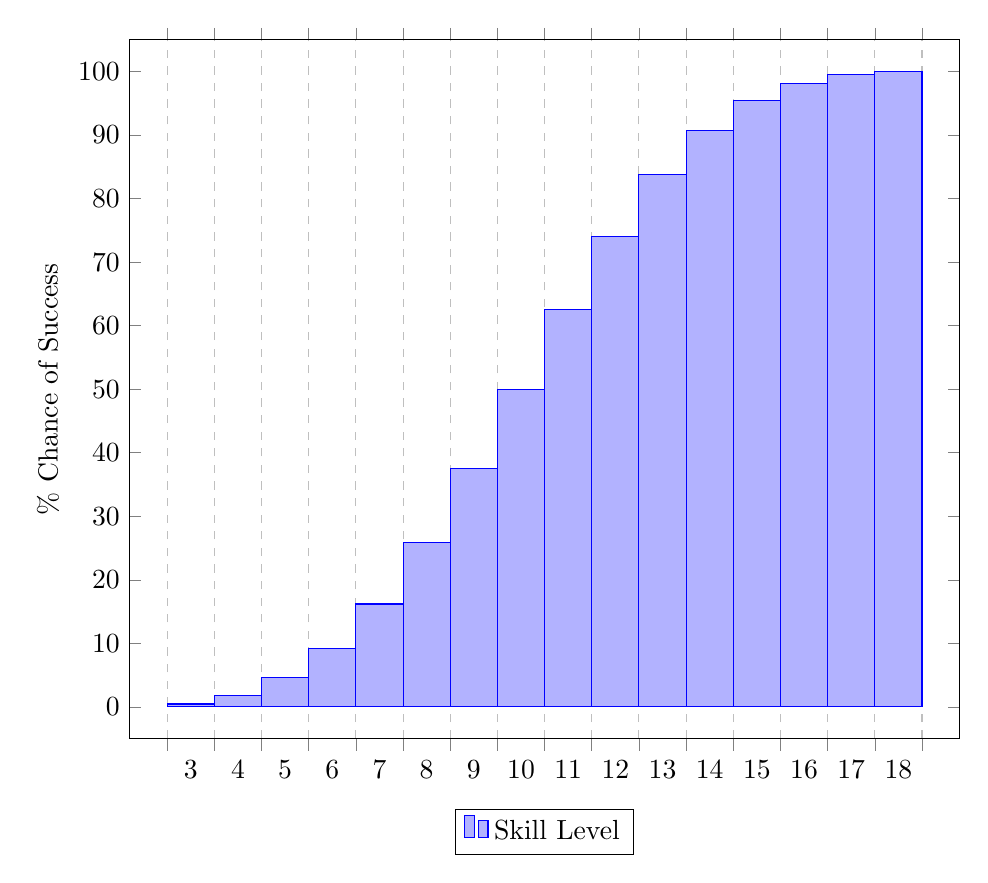
\begin{tikzpicture}
\begin{axis}[
	x tick label style={/pgf/number format/1000 sep=},
	ylabel=\% Chance of Success,
	enlargelimits=0.05,
	ytick = {0, 10, 20, 30, 40, 50, 60, 70, 80, 90, 100},
	legend style = {
	    at={(0.5,-0.1)},
	    grid style = dashed,
	    anchor=north,legend columns=-1
	},
	ybar interval = 1,
]
\addplot 
	coordinates {
	    (3,    0.46) 
	    (4,    1.85)
		(5,    4.63) 
		(6,    9.26) 
		(7,   16.20) 
		(8,   25.93) 
		(9,   37.50) 
		(10,  50.00) 
		(11,  62.50) 
		(12,  74.07)
		(13,  83.80)
		(14,  90.74)
		(15,  95.37)
		(16,  98.15)
		(17,  99.54)
		(18, 100.00)
		(19, 0)
	};
\legend{Skill Level}
\end{axis}
\end{tikzpicture}\\
The graph above shows the probability of succeeding a skill roll. If your character has an effective skill of 10, they have a 50\% chance of succeeding that roll. If they have a skill of 12, the chance of success goes up to 74\%.
\section{Critical Miss Table (Melee)}
\begin{center}
\begin{tabular}{r | l}
    \textbf{Roll} & \textbf{Result}\\\hline
    1 & Your weapon turns in your hand, and you hit with the flat side! \\
    2 & Your weapon breaks! \\
    3 & You lose your grip and the weapon flies out of your hand! \\
    4 & You lose your balance, and your turn! \\
    5 & You trip and fall! You have to get up again.\\
    6 & You hit yourself in the arm or leg! (50\% chance of hitting either)\\
\end{tabular}
\end{center}
\paragraph{Note}For \#3, the weapon flies 1d6 squares (50\% chance forward or backward). If it hits someone, it does half damage and lands there.

%% \section{Critical Miss Table (Ranged)}
%% \begin{center}
%% \begin{tabular}{r | l}
%%     \textbf{Roll} & \textbf{Result}\\\hline
%%     1 & Your weapon jams.\\
%%     2 &\\
%%     3 &\\
%%     4 &\\
%%     5 &\\
%%     6 &\\
%% \end{tabular}
%% \end{center}

\section{Weapons} \label{sec:weapons}
\subsection{Melee Weapons}
\begin{center}
\begin{tabular}{c|c|c|c|c|c}
    \textbf{Category} & \textbf{Name} & \textbf{Class} & \textbf{Damage} & \textbf{Damage Type} & \textbf{Range} \\\hline
    Unarmed  & Fists          & Light & d6-2 & Crushing & Close/1\\
             & Feet           & Light & d6-1 & Crushing & Close/1\\\hline
    Medieval & Short Sword    & Light & d6   & Slashing & Close/1\\
             & Long Sword     & Heavy & d6+2 & Slashing & 1 to 2 \\
             & Mace           & Heavy & d6+2 & Crushing & Close/1\\\hline
    Modern   & Baseball Bat   & Heavy & d6+1 & Crushing & Close/1\\
             & Aluminium Bat  & Light & d6+1 & Crushing & Close/1\\
             & Brass Knuckles & Light & d6-1 & Crushing & Close/1\\\hline
    Future   & Beam Sword     & Light & d6+3 & Slashing & Close/1
\end{tabular}
\end{center}

\subsection{Ranged Weapons}
\begin{center}
\begin{tabular}{c|c|c|c|c}
    \textbf{Category} & \textbf{Name} & \textbf{Damage} & \textbf{Damage Type} & \textbf{Accurate Range} \\\hline
    Primitive & Rock        & d6-1  & Crushing & $0.5 \times Shooting + Prof$  \\\hline
    Medieval  & Short Bow   & d6+1  & Piercing & $Shooting + Prof$ \\
              & Long Bow    & d6+2  & Piercing & $2 \times Shooting + Prof$ \\\hline
    Modern    & Pistol      & 2d6+2 & Crushing & 56m \\
              & Shotgun     & 5d6   & Crushing & 3m \\\hline
    Future    & Laser Gun   & 6d6   & Piercing & 66m \\
\end{tabular}
\end{center}
\paragraph{Note} These ranges are for when you want to shoot without a range penalty.
So despite the fact that a pistol can shoot around 1800m, it's incredibly hard to do so.

\section{Armour}
\begin{center}
\begin{tabular}{c|c|c|c}
\textbf{Category} & \textbf{Name}  & \textbf{PD} & \textbf{DR}\\\hline
         Medieval & Learther       & 1 & 1 \\
                  & Half Plate     & 2 & 2 \\
                  & Full Plate     & 4 & 3 \\
                  & Chain Mail     & 1 & 1 \\\hline
           Modern & Summer Clothes & 0 & 0 \\
                  & Winter Clothes & 0 & 1 \\
                  & Kevlar Vest    & 1 & 3 \\\hline
           Future & Polymer        & 4 & 3 \\
\end{tabular}
\end{center}

\chapter{Character Sheets}\label{app:character-sheets}
This Appendix contains some example character sheets as well as an empty one ready for printout.
\includepdf[pages = -]{graphics/character-sheet-example.pdf}
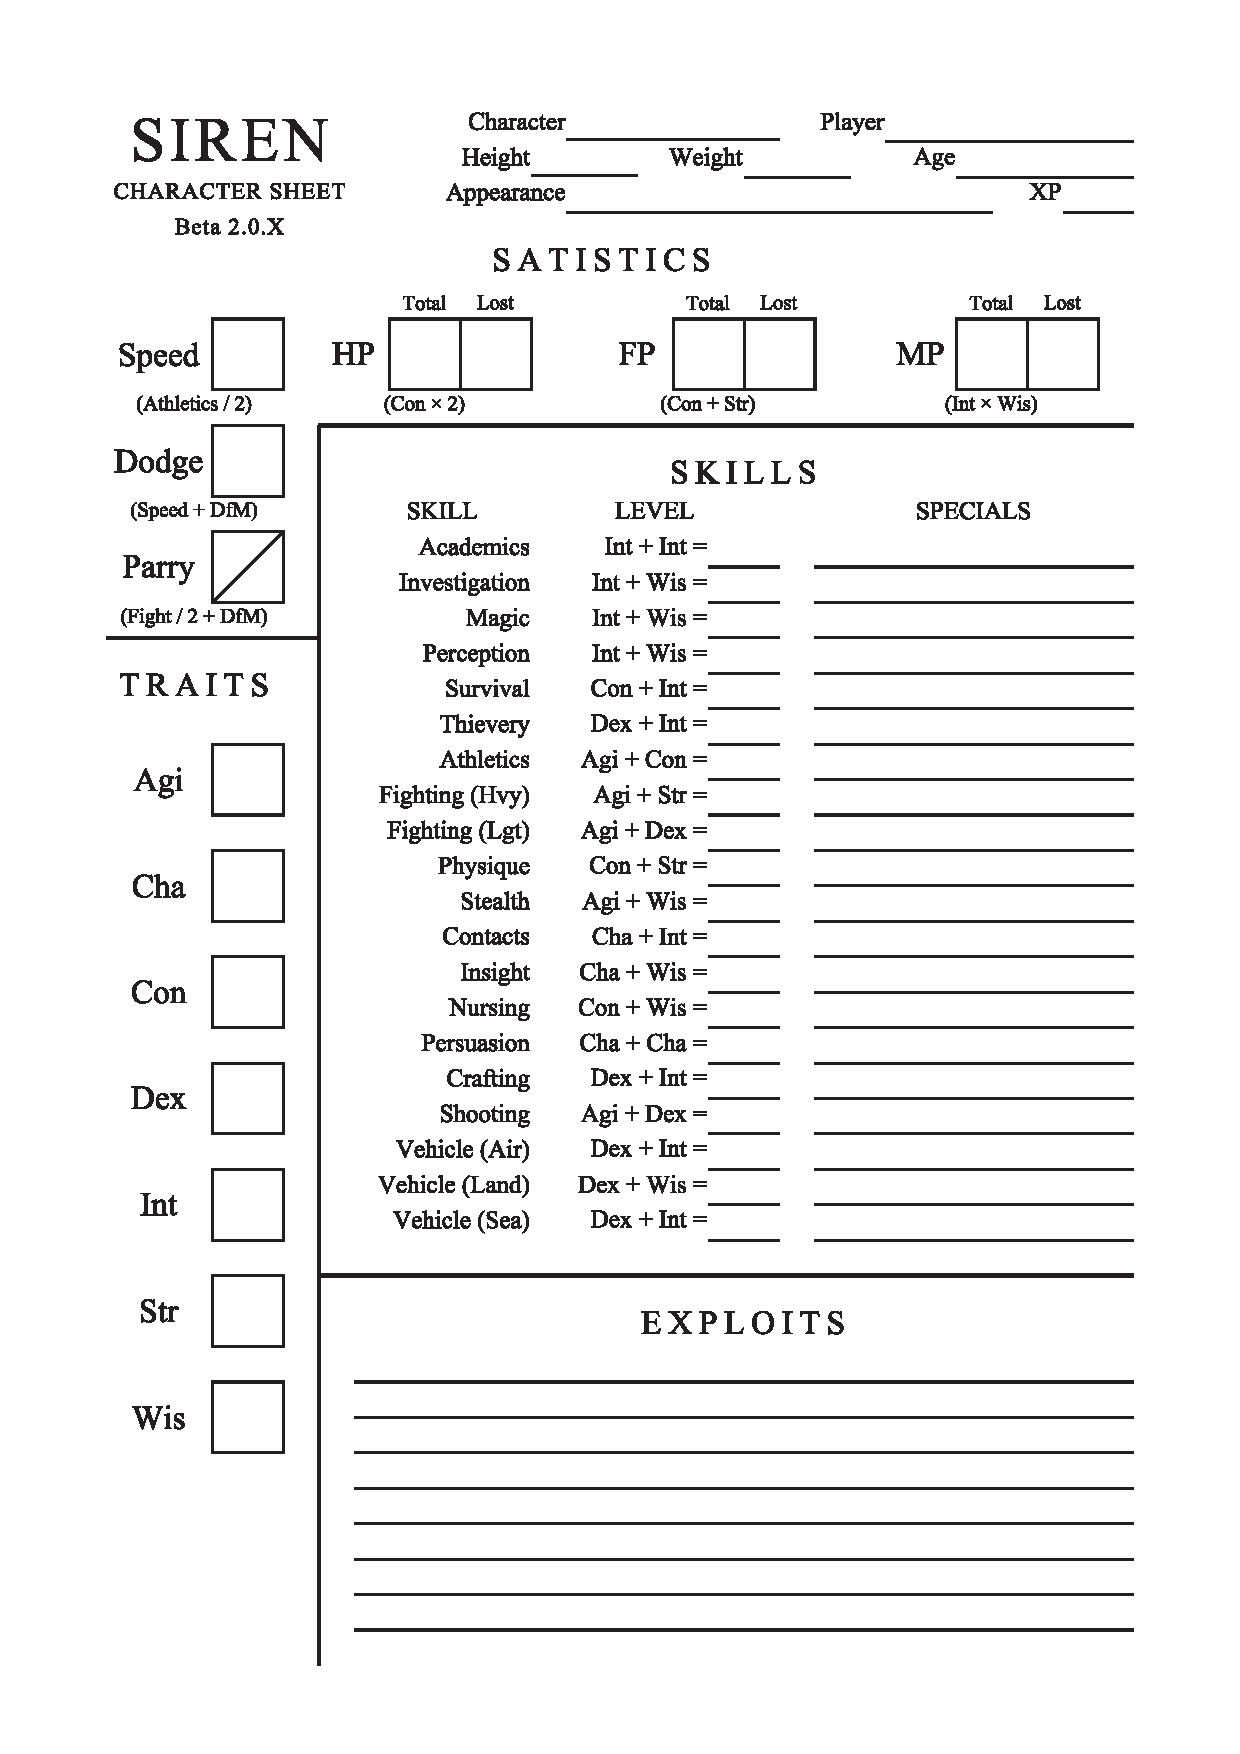
\includepdf[pages = -]{graphics/siren-character-sheet.pdf}
\end{document}
